\chapter{Analyse af ISO226}
\label{AnalyseAfISO226}
%
Følgende afsnit fokuserer på en grundigere analyse af \textit{Normal Equal-Loudness-Level Contours}, som er fremsat i \textcite{STD:ISO226}. Formålet er at analysere, om der er en sammenhæng mellem de syv forskellige phon-kurver i forhold til referencen. Referencen fastsættes til 80phon fordi der ved vedvarende støjbelastning over 80dB(A) vil være en forøget risiko for at udvikle høreskader, \parencite[s. 4]{PDF:ATVejledning}. Ved en reference fastsat til 80phon, resulterer det i at ved 1000Hz, perciperes den som værende 80dB, hvilket resulterer i et \textit{Loudness Level} på 80phon. At referencen vælges til 80phon skyldes at der  Ved at analysere denne sammenhæng vil det være muligt at blotlægge ændringerne i de specifikke phon-kurvers hældning sammenlignet med referencen. Derfra kan det konkluderes hvorvidt tonerne ved de forskellige frekvenser enten skal forstærkes eller dæmpes, for at opnå en tilsvarende perception, som hvis tonen afspilles ved referencen, blot x-antal dB lavere. Yderligere vil det blive analyseret, hvorvidt der forekommer ændringer afhængigt af om det er lav-, mellem- og højfrekvente toner. \\[5mm]
%
Analysen fokuserer på data tilhørende phon-kurverne fra 20phon til 90phon, som spænder over frekvensområdet fra 20Hz til 12500Hz, dog med forbehold for at data tilhørende 90phon kun spænder over frekvensområdet fra 20Hz til og med 4000Hz, jævnfør \fullref{ISO226}. Frekvensområdet er defineret i \textcite[s. 1]{STD:ISO226}, som værende en tredjedel oktav mellem 20Hz og 12500Hz, hvor de specifikke frekvensværdier fremgår af Table B.1 i \textcite[ss. 6-7]{STD:ISO226}. Det data der vil blive analyseret repræsenterer således forholdet mellem lydtryksniveauer og \textit{Loudness Level} for rene toner i det opgivne frekvensområde, data fremgår af \autoref{app:ISO226Raadata}.

For at analysere sammenhængen mellem phon-kurverne udregnes der for hver phon-kurve en difference mellem dennes datapunkter og referencens datapunkter. Først udregnes en forskydningsfaktor, som er differencen mellem referencen og den specifikke phon-kurve, differencen angives i dB. Dertil subtraheres differencen mellem referencens lydtryksniveau og den specifikke phon-kurves lydtryksniveau, målt ved den pågældende frekvens. Denne procedure udføres for samtlige datapunkter, hvoraf resultatet definerer et nyt datasæt bestående af differencen mellem referencen og hver af de syv phon-kurver, angivet i dB. Datapunkterne udregnes ved følgende ligning: 
%
\begin{equation}
	datapunkt=(phon_{ref}-phon_{level})-(dB_{ref}-dB_{level})
\label{equ:DifDatapunkt}
\end{equation}
\noindent
%
Hvor:
%
\begin{itemize}
	\item[] $phon_{ref}$ er referencen på 80phon
	\item[] $phon_{level}$ er den specifikke phon-kurve, hvorfra differencen skal findes
	\item[] $dB_{ref}$ er referencens lydtryksniveau målt ved den pågældende frekvens
	\item[] $dB_{level}$ er den specifikke phon-kurves lydtryksniveau målt ved den pågældende frekvens\\[5mm]
\end{itemize}
\noindent
%
Et datapunkt til det nye datasæt udregnes eksempelvist ved at tage forskydningsfaktoren, der er differencen mellem referencen og den specifikke phon-kurve, som er 20phon, og subtrahere differencen mellem lydtryksniveauet målt ved 20Hz tilhørende referencen med det tilsvarende lydtryksniveau målt ved 20phon, hvilket giver følgende udregning:
%
\begin{equation}
	(80-20)-(119-89.6)=30.6
\end{equation}      
\noindent
%
Resultatet indikerer at hvis en 20Hz tone afspilles ved 20phon, så skal tonen forstærkes med 30.6dB for at blive perciperet på samme måde, som hvis tonen blev afspillet ved referencen, blot 60dB lavere. I det her tilfælde er forskydningsfaktoren 60dB. En positiv difference angiver at tonen skal forstærkes, hvor en negativ difference angiver at tonen skal dæmpes. De resterende datapunkter i det nye datasæt fremgår af \autoref{app:ISO226Difference}.  
%
\begin{figure}[H]
	\centering
	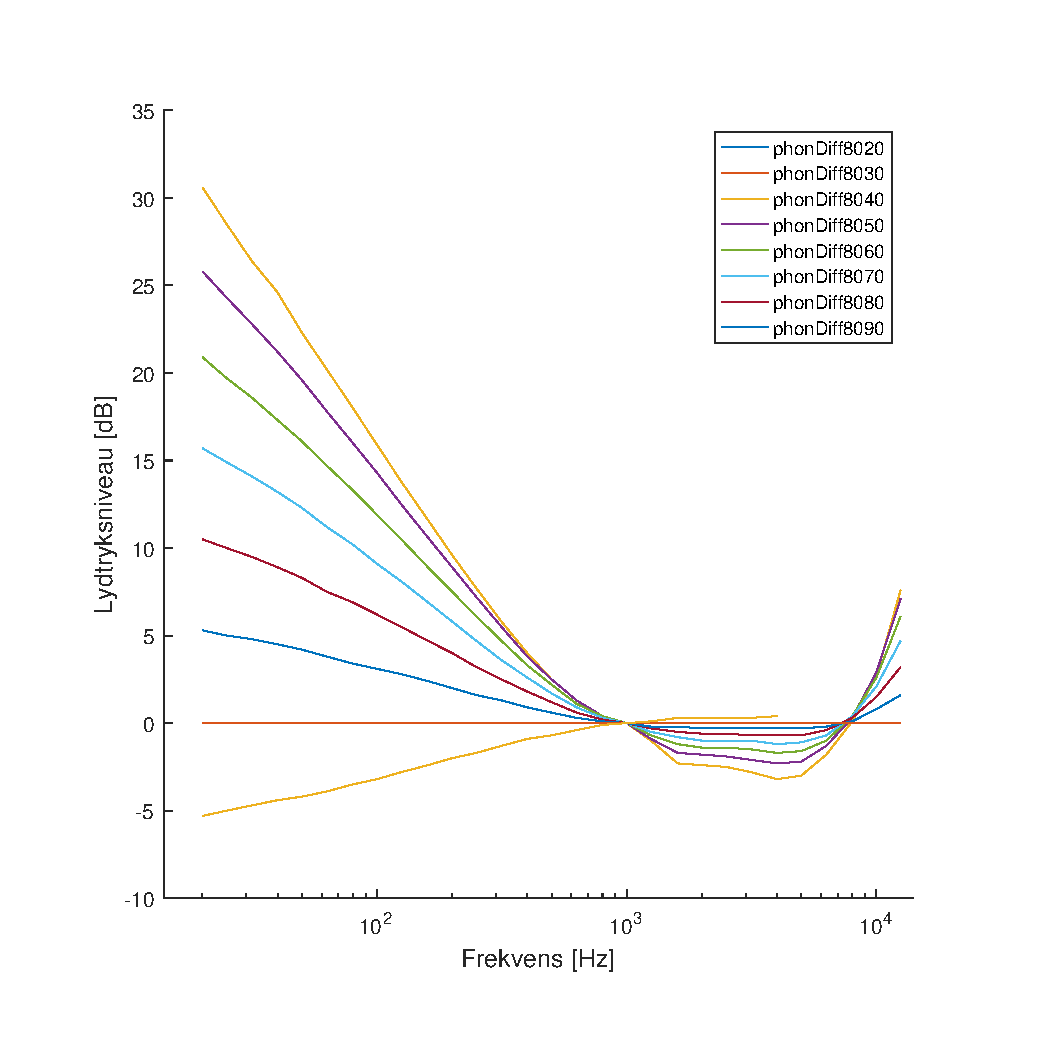
\includegraphics[resolution=300,width=\textwidth]{Introduktion/ISO226Difference.pdf}
	\caption{Semilogaritmisk afbildning af det nye datasæt, hvor den logaritmiske x-akse angiver frekvens i hertz og den lineære y-akse angiver lydtryksniveau i dB, som udregnes via \autoref{equ:DifDatapunkt}.}
	\label{fig:DifferenceKurver}
\end{figure}
\noindent
%
På \autoref{fig:DifferenceKurver} fremgår det hvornår en tone enten skal forstærkes eller dæmpes afhængigt af hvilken phon-kurve der følges, samt hvilken frekvens tonen har. Dertil kan det fastsættes at så længe tonerne ikke tilhører 90phon-kurven og samtidig er under 1000Hz så skal de forstærkes, modsat skal toner under 1000Hz, der følger 90 phon-kurven, dæmpes. For at afgøre hvorvidt det er nødvendigt at kompensere for menneskets perception af toner, er det favorabelt at inddrage \textit{Just Noticeable Difference}, JND, i forhold til detektering af intensitetsforskelle vedrørende \textit{Loudness}. Hvor intensitetsforskelle angiver forskelle i lydtryksniveauer. Med udgangspunkt i \textit{Weber fraction}, som er forholdet mellem $\Delta I$ og $I$, hvor $\Delta I$ er den mindste perciperede ændring i intensitet og $I$ er intensiteten af tonen, hvor forholdet antages for at være konstant, \parencite[s. 60]{BOOK:AnIntroductionToThePsycologyOfHearing}. Såfremt forholdet skal angives i dB vil forholdet blive udregnet ved: 
%
\noindent
\begin{equation}
	\Delta L= 10*log\left[\frac{(I+\Delta I)}{I}\right]
\label{equ:JND}
\end{equation}
\noindent
%
$\Delta L$ angiver JND for den hørbare ændring i \textit{Loudness}, som for \textit{Wideband Noise} er mellem 0.5dB og 1dB for lydtryksniveauer mellem 20dB og 100dB, \parencite[s. 60]{BOOK:AnIntroductionToThePsycologyOfHearing}. \textit{Wideband Noise} er støj over et stort område af frekvenser i det hørebare spektrum. Problemet med at tage udgangspunkt i \textit{Weber Fraction} er, at den ikke gør sig gældende for rene toner, hvilket er det der bliver undersøgt i \textcite{STD:ISO226}. Derimod kan der tages udgangspunkt i \textcite[s. 774]{PDF:OnTheRelationsOfIntensityJND}, hvis data afbilledes på \autoref{fig:RieszJND}, som angiver JND for 1000Hz ved lydtryksniveauer fra 10dB til 90dB.
%
\begin{figure}[H]
	\centering
	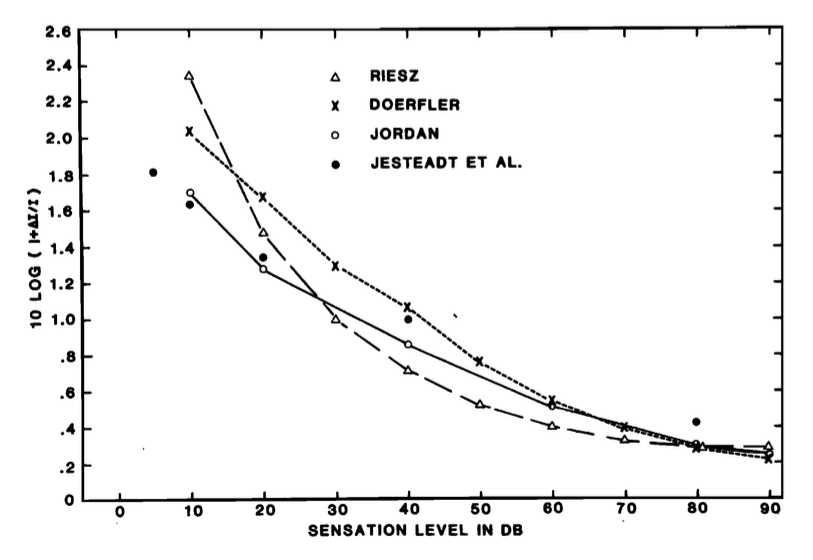
\includegraphics[resolution=300,width=\textwidth]{Introduktion/RieszJND.png}
	\caption{Der fokuseres udelukkende på Riesz's data, som repræsenteres med $\triangle$. Akserne angives ved lydtryksniveau i dB på x-aksen og JND, som er udregnet ved \autoref{equ:JND}, på y-aksen, \parencite[s. 774]{PDF:OnTheRelationsOfIntensityJND}.}
	\label{fig:RieszJND}
\end{figure}
\noindent
%
Med udgangspunkt i \autoref{fig:DifferenceKurver} forefindes den største difference mellem 20phon og referencen ved 20Hz, hvor differencen er 30.6dB. For at der ikke er en hørbar forskel mellem 20phon og 30phon ved 20Hz skal differencen mellem dem, ifølge \autoref{fig:RieszJND}, være omkring 1dB til 1.5dB, hvilket ikke er tilfældet, da differencen er 4.8dB, jævnfør \autoref{app:ISO226Difference}. 

Da de resterende phon-kurver repræsenteres med en difference fra 20.9dB og ned, tages der udgangspunkt i JND for 20dB ved 1000Hz, som ifølge \autoref{fig:RieszJND} og \textcite[s. 61]{BOOK:AnIntroductionToThePsycologyOfHearing}, er 1.5dB.\\[5mm]
%
For at afgøre hvorvidt det er nødvendigt at forstærke eller dæmpe tonerne skal differencen mellem de individuelle phon-kurver og referencen på 80phon ved 1000Hz være $\pm 1.5$dB. Det er derfor muligt at angive én frekvens under 1000Hz, hvor tonerne ikke længere perciperes som værende af forskellige lydtryk, uafhængigt af phon-kurverne. Frekvensen vælges baseret på \autoref{app:ISO226Difference}, ved at addere JND, 1.5dB, til referencen, 1000Hz, hvilket resulterer i at den valgte frekvens er 630Hz. Men da der forekommer små afvigelser vedrørende lydtryksniveauerne målt ved de lave frekvenser, afhængigt af hvilken phon-kurve der tages udgangspunkt i, er det fordelagtigt at hæve grænsen til 1000Hz fremfor 630Hz.

Sammenholdes \autoref{fig:DifferenceKurver} med det tilhørende datasæt \autoref{app:ISO226Difference}, i frekvensområdet fra 800Hz til og med 8000Hz, tyder det på at det vil være unødvendigt at foretage ændringer, da differencen mellem de specifikke phon-kurver og referencen er uhørbar, \parencite[s. 60]{BOOK:AnIntroductionToThePsycologyOfHearing}. Ligeledes vil det for frekvensområdet mellem 10000Hz og 12500Hz være unødvendigt at foretage ændringer, da differencen, i det fleste tilfælde, er minimal.\\[5mm]
%
Fremadrettet vil der derfor kun fokuseres på frekvensområdet mellem 20Hz og 1000Hz, som ydermere defineres som værende det lavfrekventeområde. I relation til problemformuleringen, \fullref{Problemformulering}, og baseret på den foregående analyse, afgrænses der til kun at kompensere for mennesket frekvensafhængige perception af lydtryksniveauer i det lavfrekventeområde. Følgende kapitler vil fokusere på hvordan en elektronisk løsning, ved brug af analogteknik, kan udarbejdes.

